\documentclass{beamer}
\usepackage[utf8]{inputenc}

\usetheme{Madrid}
\usecolortheme{default}
\usepackage{amsmath,amssymb,amsfonts,amsthm}
\usepackage{txfonts}
\usepackage{tkz-euclide}
\usepackage{listings}
\usepackage{adjustbox}
\usepackage{array}
\usepackage{tabularx}
\usepackage{gvv}
\usepackage{lmodern}
\usepackage{circuitikz}
\usepackage{tikz}
\usepackage{graphicx}

\setbeamertemplate{page number in head/foot}[totalframenumber]

\usepackage{tcolorbox}
\tcbuselibrary{minted,breakable,xparse,skins}

\definecolor{bg}{gray}{0.95}
\DeclareTCBListing{mintedbox}{O{}m!O{}}{%
  breakable=true,
  listing engine=minted,
  listing only,
  minted language=#2,
  minted style=default,
  minted options={%
    linenos,
    gobble=0,
    breaklines=true,
    fontsize=\small,
    numbersep=8pt,
    #1},
  boxsep=0pt,
  left skip=0pt,
  right skip=0pt,
  left=25pt,
  right=0pt,
  top=3pt,
  bottom=3pt,
  arc=5pt,
  leftrule=0pt,
  rightrule=0pt,
  bottomrule=2pt,
  toprule=2pt,
  colback=bg,
  colframe=orange!70,
  enhanced,
  overlay={%
    \begin{tcbclipinterior}
    \fill[orange!20!white] (frame.south west) rectangle ([xshift=20pt]frame.north west);
    \end{tcbclipinterior}},
  #3,
}

\lstset{
    language=C,
    basicstyle=\ttfamily\small,
    keywordstyle=\color{blue},
    stringstyle=\color{orange},
    commentstyle=\color{green!60!black},
    numbers=left,
    numberstyle=\tiny\color{gray},
    breaklines=true,
    showstringspaces=false,
}

%------------------------------------------------------------
% Title info
\title{2.7.21}
\date{September 14, 2025}
\author{Anshu kumar ram-EE25BTECH11009}

\begin{document}

\frame{\titlepage}

% ---------------- Question ----------------
\begin{frame}{Question}
Find the values of $k$ so that the area of the triangle with vertices 
$A(1,-1),\; B(-4,2k),\; C(-k,-5)$ is $24$ sq. units.
\end{frame}

% ---------------- Step 1 ----------------
\begin{frame}{Step 1: Vertices}
\begin{table}[h!]
    \centering
    \begin{tabular}{|c|c|}
        \hline
        Point & Coordinates \\
        \hline
	    $A$ & $\myvec{1\\-1}$ \\
	    $B$ & $\myvec{-4\\2k}$ \\
	    $C$ & $\myvec{-k\\-5}$ \\
        \hline
    \end{tabular}
    \caption{Vertices of $\triangle ABC$ before substituting $k$}
    \label{tab:triangle_k}
\end{table}

\end{frame}

% ---------------- Step 2 ----------------
\begin{frame}{Step 2: Vectors}
\begin{align}
\vec{u} &= \vec{B}-\vec{A} = \myvec{-5 \\ 2k+1}, \\
\vec{v} &= \vec{C}-\vec{A} = \myvec{-k-1 \\ -4}
\end{align}

\begin{align}
\Delta &= \frac{1}{2}\|\vec{u}\times \vec{v}\|
\end{align}
\end{frame}

% ---------------- Step 3 ----------------
\begin{frame}{Step 3: Norm Identity}
\begin{align}
\|\vec{u}\times\vec{v}\|^2 
&= \|\vec{u}\|^2 \|\vec{v}\|^2 - (\vec{u}^\top\vec{v})^2
\end{align}
\begin{align}
\implies \|\vec{u}\times\vec{v}\| &= |2k^2+3k+21|
\end{align}
\begin{align}
\Delta &= \frac{1}{2}|2k^2+3k+21|
\end{align}
\end{frame}

% ---------------- Step 4 ----------------
\begin{frame}{Step 4: Solve for $k$}
\begin{align}
\frac{1}{2}|2k^2+3k+21| &= 24 \\
|2k^2+3k+21| &= 48
\end{align}

Case 1:
\begin{align}
2k^2+3k-27=0 \;\;\implies\; k=3,\; -\tfrac{9}{2}
\end{align}

Case 2:
\begin{align}
2k^2+3k+69=0 \;\; \text{(no real roots)}
\end{align}
\end{frame}

% ---------------- Step 5 ----------------
\begin{frame}{Step 5: Final Answer}
\begin{align}
\therefore k \in \{3,\; -\tfrac{9}{2}\}
\end{align}

\begin{table}[h!]
    \centering
    \begin{tabular}{|c|c|c|}
        \hline
        Point & For $k=3$ & For $k=-\tfrac{9}{2}$ \\
        \hline
        $A$ & $\myvec{1\\-1}$ & $\myvec{1\\-1}$ \\
$B$ & $\myvec{-4\\6}$ & $\myvec{-4\\-9}$ \\
$C$ & $\myvec{-3\\-5}$ & $\myvec{\tfrac{9}{2}\\-5}$ \\
        \hline
    \end{tabular}
    \caption{Vertices of $\triangle ABC$ after substituting $k$ values}
    \label{tab:triangle_values}
\end{table}

\end{frame}

% ---------------- Graph ----------------
\begin{frame}{Graph}
\centering
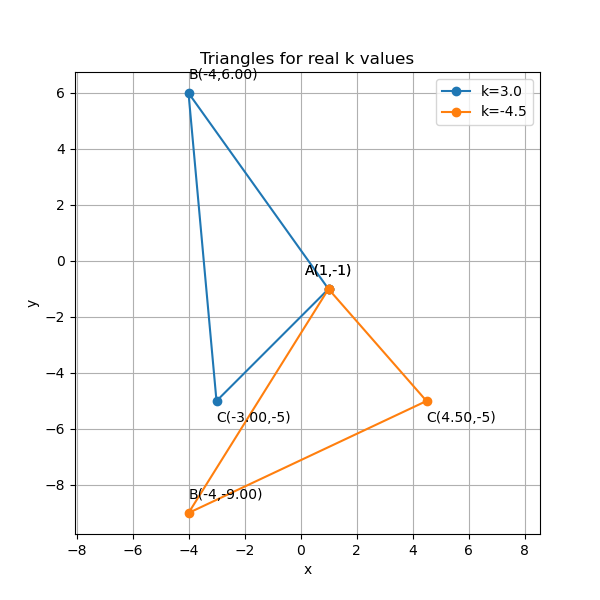
\includegraphics[width=0.75\linewidth]{./figs/triangle_area.png}

\bigskip
Vertices: 
$\boldsymbol{A}(1,-1),\;
 \boldsymbol{B}(-4,2k),\;
 \boldsymbol{C}(-k,-5)$
\end{frame}


% ---------------- C Code ----------------
\begin{frame}[fragile]{C Code (Part 1)}
\begin{lstlisting}
#include <stdio.h>
#include <math.h>

// Function to compute area of a triangle given coordinates
double triangle_area(double *A, double *B, double *C) {
    // A, B, C are arrays of size 2: [x, y]
    double x1 = A[0], y1 = A[1];
    double x2 = B[0], y2 = B[1];
    double x3 = C[0], y3 = C[1];
\end{lstlisting}
\end{frame}

\begin{frame}[fragile]{C Code (Part 2)}
\begin{lstlisting}
    // Determinant method for area
    double det = x1*(y2 - y3) + x2*(y3 - y1) + x3*(y1 - y2);
    return fabs(det) / 2.0;
}

/* Build as shared library:
   gcc -fPIC -shared -o func.so func.c
*/
\end{lstlisting}
\end{frame}

% ---------------- Python + C ----------------
\begin{frame}[fragile]{Python + C (Part 1)}
\begin{lstlisting}
import ctypes
import numpy as np
import matplotlib.pyplot as plt

# Load shared library
handc = ctypes.CDLL("./func.so")

# Define argument and return types for the C function
handc.triangle_area.argtypes = [
    ctypes.POINTER(ctypes.c_double),  # A
    ctypes.POINTER(ctypes.c_double),  # B
    ctypes.POINTER(ctypes.c_double)   # C
]
handc.triangle_area.restype = ctypes.c_double
\end{lstlisting}
\end{frame}

\begin{frame}[fragile]{Python + C (Part 2)}
\begin{lstlisting}
# Convert numpy arrays to C pointers
def np_to_c(arr):
    return arr.ctypes.data_as(ctypes.POINTER(ctypes.c_double))

# Fixed point A
A = np.array([1.0, -1.0], dtype=np.float64)

# k values we found
k_vals = [3.0, -9.0/2.0]
plt.figure(figsize=(6,6))
\end{lstlisting}
\end{frame}

\begin{frame}[fragile]{Python + C (Part 3)}
\begin{lstlisting}
for k in k_vals:
    B = np.array([-4.0, 2.0*k], dtype=np.float64)
    C = np.array([-k, -5.0], dtype=np.float64)
    
    # Call the C function for area
    area = handc.triangle_area(np_to_c(A), np_to_c(B), np_to_c(C))
    print(f"k = {k}, area = {area}")
    
    # Plot triangle
    x_coords = [A[0], B[0], C[0], A[0]]
    y_coords = [A[1], B[1], C[1], A[1]]
    plt.plot(x_coords, y_coords, marker='o', label=f"k={k}")
\end{lstlisting}
\end{frame}

\begin{frame}[fragile]{Python + C (Part 4)}
\begin{lstlisting}
    # Plot points with labels
    plt.scatter([A[0], B[0], C[0]], [A[1], B[1], C[1]], s=50)
    plt.annotate("A(1,-1)", (A[0], A[1]), textcoords="offset points", xytext=(0,10), ha='center')
    plt.annotate(f"B(-4,{2*k:.1f})", (B[0], B[1]), textcoords="offset points", xytext=(0,10))
    plt.annotate(f"C({-k:.1f},-5)", (C[0], C[1]), textcoords="offset points", xytext=(0,-15))

plt.xlabel("x")
plt.ylabel("y")
plt.title("Triangles (Python + C area function)")
plt.legend()
plt.axis("equal")
plt.grid(True)
plt.savefig("../figs/triangle_area_c.png")
plt.show()
\end{lstlisting}
\end{frame}

% ---------------- Pure Python ----------------
\begin{frame}[fragile]{Pure Python (Part 1)}
\begin{lstlisting}
import math
import sys
sys.path.insert(0, '/home/anshu-ram/matgeo/codes/CoordGeo')
import numpy as np
import numpy.linalg as LA
import matplotlib.pyplot as plt

# Given vertex A
A = np.array([1.0, -1.0]).reshape(-1,1)

# Real k solutions found
k_vals = [3.0, -9.0/2.0]
plt.figure(figsize=(6,6))
\end{lstlisting}
\end{frame}

\begin{frame}[fragile]{Pure Python (Part 2)}
\begin{lstlisting}
for k in k_vals:
    B = np.array([-4.0, 2.0*k]).reshape(-1,1)
    C = np.array([-k, -5.0]).reshape(-1,1)
    
    tri = np.hstack((A, B, C, A))
    plt.plot(tri[0,:], tri[1,:], linestyle='-', marker='o', label=f'k={k}')
    
    # area using cross product
    u = (B - A).flatten()
    v = (C - A).flatten()
    cross = abs(u[0]*v[1] - u[1]*v[0])
    area = 0.5*cross
    print(f"k={k} => computed area = {area}")
\end{lstlisting}
\end{frame}

\begin{frame}[fragile]{Pure Python (Part 3)}
\begin{lstlisting}
    # annotate vertices
    plt.annotate(f'A(1,-1)', (A[0,0], A[1,0]), textcoords="offset points", xytext=(0,10), ha='center')
    plt.annotate(f'B(-4,{2*k:.2f})', (B[0,0], B[1,0]), textcoords="offset points", xytext=(0,10))
    plt.annotate(f'C({-k:.2f},-5)', (C[0,0], C[1,0]), textcoords="offset points", xytext=(0,-15))

plt.xlabel('x')
plt.ylabel('y')
plt.title('Triangles for real k values')
plt.legend()
plt.axis('equal')
plt.grid(True)
plt.savefig("../figs/triangle_area.png")
plt.show()
\end{lstlisting}
\end{frame}

\end{document}
